\uuid{9Bs3}
\exo7id{5539}
\titre{exo7 5539}
\auteur{rouget}
\organisation{exo7}
\datecreate{2010-07-15}
\isIndication{false}
\isCorrection{true}
\chapitre{Courbes planes}
\sousChapitre{Propriétés métriques : longueur, courbure,...}
\module{Géométrie}
\niveau{L2}
\difficulte{}

\contenu{
\texte{
Pour $\lambda\in\Rr$, on note $(\Gamma_\lambda)$ la courbe d'équation $y=\lambda xe^{-x}$. Quel est le lieu des centres de courbure $C_\lambda$ en $O$ à $(\Gamma_\lambda)$ quand $\lambda$ décrit $\Rr$.
}
\reponse{
Soit $\lambda\in\Rr$. $\mathcal{C}_\lambda$ est le support de l'arc paramétré $t\mapsto\left(
\begin{array}{c}
t\\
\lambda te^{-t}
\end{array}
\right)$. $\mathcal{C}_0$ est l'axe $(Ox)$ et donc $C_0$ n'est pas défini, puis $\mathcal{C}_{-\lambda}$ est la symétrique de $\mathcal{C}_\lambda$ par rapport à l'axe $(Ox)$ et donc $C_{-\lambda}$ est le symétrique de $C_\lambda$ par rapport à l'axe $(Ox)$. Dans ce qui suit, on suppose $\lambda>0$.

\begin{center}
$\overrightarrow{\frac{dM}{dt}}=\left(
\begin{array}{c}
1\\
\lambda(1-t)e^{-t}
\end{array}
\right)$.
\end{center}
Par suite $\frac{ds}{dt}=\sqrt{1+\lambda^2(1-t)^2e^{-2t}}$, $\overrightarrow{\tau}(t)=\frac{1}{\sqrt{1+\lambda^2(1-t)^2e^{-2t}}}\left(
\begin{array}{c}
1\\
\lambda(1-t)e^{-t}
\end{array}
\right)$,

$\overrightarrow{n}(t)=\frac{1}{\sqrt{1+\lambda^2(1-t)^2e^{-2t}}}\left(
\begin{array}{c}
-\lambda(1-t)e^{-t}\\
1
\end{array}
\right)$ et on peut prendre $\alpha(t)=\Arccos\left(\frac{1}{\sqrt{1+\lambda^2(1-t)^2e^{-2t}}}\right)$ (car $\overrightarrow{\tau}(t)$ a une abscisse strictement positive). Ensuite,

\begin{center}
$\frac{d\alpha}{dt}=\frac{\lambda^2((2t-2)-2(t-1)^2)e^{-2t}}{2(1+\lambda^2(1-t)^2e^{-2t})^{3/2}}\frac{1}{\sqrt{1-\frac{1}{1+\lambda^2(1-t)^2e^{-2t}}}}$
\end{center}
et donc $\frac{d\alpha}{dt}(0)=\frac{-4\lambda^2}{2(1+\lambda^2)^{3/2}}\frac{1}{\sqrt{1-\frac{1}{1+\lambda^2}}}=\frac{-2\lambda}{1+\lambda^2}$ puis $R(0)=\frac{ds/dt}{d\alpha/dt}(0)=-\frac{1}{2\lambda}(1+\lambda^2)^{3/2}$ et donc

\begin{center}
$C_\lambda=\Omega(0)=M(0)+R(0)\overrightarrow{n}(0)=O-\frac{1}{2\lambda}(1+\lambda^2)^{3/2}\frac{1}{\sqrt{1+\lambda^2}}\left(
\begin{array}{c}
-\lambda\\
1
\end{array}
\right)=\left(
\begin{array}{c}
(1+\lambda^2)/2\\
-(1+\lambda^2)/(2\lambda)
\end{array}
\right).$
\end{center}
L'ensemble des $C_\lambda$, $\lambda\in\Rr^*$, est le support de l'arc $\lambda\mapsto\left(
\begin{array}{c}
(1+\lambda^2)/2\\
-(1+\lambda^2)/(2\lambda)
\end{array}
\right)$, $\lambda\in\Rr^*$.

$$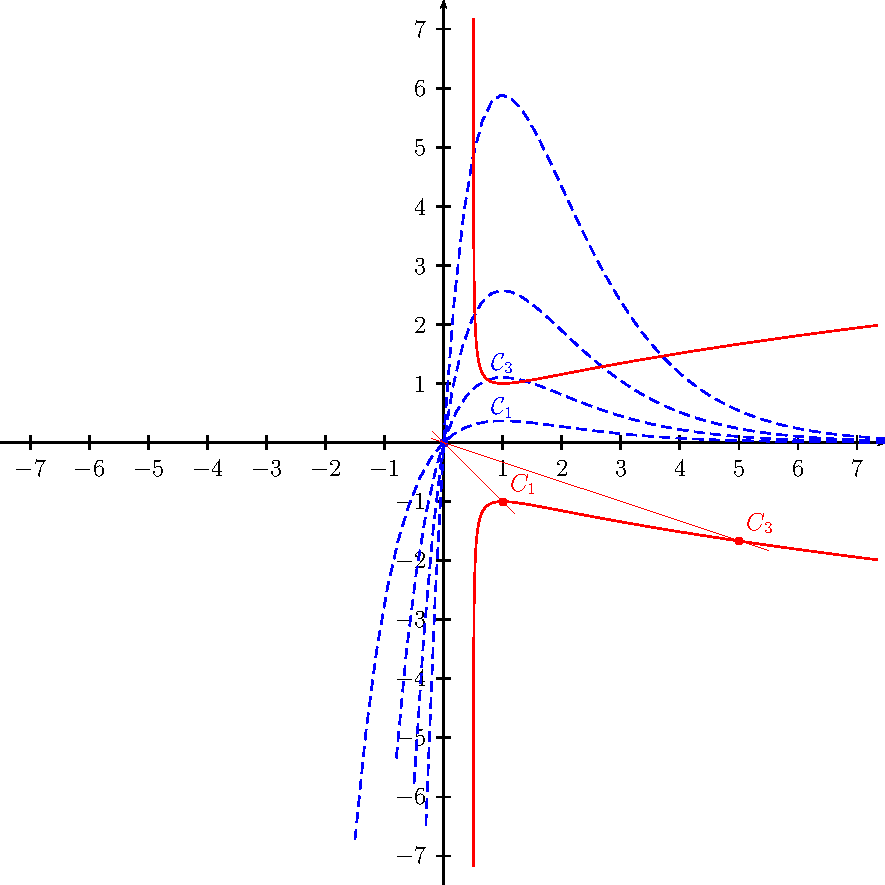
\includegraphics{../images/pdf/9Bs3-1.pdf}$$
}
}
